
\documentclass{llncs}

\usepackage{graphicx}
\usepackage{url}
\usepackage{algorithm2e}
\usepackage{amsmath,amssymb}

\begin{document}

%\conferenceinfo{WXYZ '05}{date, City.} 
%\copyrightyear{2011} 
%\copyrightdata{[to be supplied]} 

%\titlebanner{DRAFT---Do not distribute}        % These are ignored unless
%\preprintfooter{short description of paper}   % 'preprint' option specified.

 \newcommand{\assign}{$\,$:=$\;$}
\newcommand{\barc}{Barelogic$^S$}
\newcommand{\pling}{{\tt plingeling}}

\title{Performance of Parallel SAT Solvers}
\titlerunning{Parallel SAT}
\toctitle{Parallel SAT}
%\subtitle{Subtitle Text, if any, or comment out}

\author{Roberto As\'in Ach\'a\inst{1} \and Juan Olate \inst{2} \and Leo Ferres \inst{2}}

\institute{Department of Computer Engineering\\
  Faculty of Engineering\\ Universidad Cat\'olica de la Sant\'isima
  Concepci\'on, Chile\\ \email{rasin@ucsc.cl} \and Department of
  Computer Science\\Faculty of Engineering\\Universidad de
  Concepci\'on, Chile\\ \email{\{lferres|juanolate\}@udec.cl}}


\maketitle

\begin{abstract}
This is the text of the abstract.
\end{abstract}

\section{Introduction}

In this paper, we study issues of scalability of parallel solvers of
the satisfiability (SAT) problem on hierarchical-memory multicore
(SMP) systems. We find this topic important for three reasons.

Since at least 2009, parallel SAT solvers (henceforth, pSATs) have
been performing at the top of the SAT Competition (in 2011, all three
wall-clock time winners of the competition are parallel solvers).
Also in 2011, pSATs and sequential SAT solvers are grouped into a
single competition
track\footnote{\url{http://www.satcompetition.org/}}, which signals
the widespread interest in pSATs by the research and industrial
communities. This appeal stems in part because of the inherent
interesting properties of parallel algorithms, but also because of the
need of the community to do better in other application domains and be
able to handle even larger and more complex CNF formulas in smaller
times taking advantage of modern hardware.

Meanwhile, instead of increasing clock performance, chip manufacturers
are investing heavily on multicore architectures to improve
performance and lower power consumption (AMD released the 8-core
Opteron 3260 EE in late 2011, and Intel will do the same with the Xeon
E5-2650, and its low power version, the Xeon E5-2650L early this
year). As Herb Sutter once put it, ``the free lunch is over''
\cite{FreeLunchIsOver}, and this has effectively meant that software
in general will not be getting any faster as years go by simply
relying on faster processors, but by relying on how software scales in
multicore systems.

Finally, modern memory architectures are not flat
Processor$\leftrightarrow$RAM architectures, but a hierarchy of
faster-but-smaller to slow-but-large memories with latencies varying
from 0.5{\it ns} access, 32{\it Kb} memories such as the L1 cache, to
tens of nanoseconds, megabyte-large memories like the L3 cache, to
gigabyte, 100{\it ns} access memory such as main memory. Hierarchical
memory architectures have a strong impact on the performance of
sequential software (e.g., row scanning arrays in row-major
representation, memory transfers may be in the order of the input
divided by the size of the cache line, while memory transfers for
column scanning is in the order of the square of the input). % For
% multicore systems, besides the problem of data representation, there
% is the problem of false sharing: if two threads write on different
% words of the same cache line, then the cache line in one or the other
% processor becomes ``dirty'' and a round trip to RAM ensues, wasting
% valuable time due to latency.

Thus, given the three arguments above: how {\em do} pSATs scale in
hierarchical-memory multicore architectures? Our case study is the
winner of the 2011 SAT Competition, {\tt plingeling}, a
portfolio-approach SAT solver \cite{lingeling}. The first experiment
tested a \emph{modified} \pling\ on a 6-core multicore machine,
varying the number of threads. This instance of \pling\ was modified
in order that, for each {\em worker thread}, the {\em same search}
would be performed (i.e. same strategies, starting parameters and
without lemma exchanging). This allows us to measure the impact of
running $p$ threads on the same physical CPU. In Figure
\ref{fig:decay} we can see now how the modified-\pling's performance
tends to decay sharply (up to 30\%) when several instances are
executed on the same processor, even when they do not, in principle,
share any resources other than the common process address space. We
would thus expect that all instances would perform similarly, plus or
minus a small time fraction. This is in fact what happens when \pling\
is run in two different cores of two different chips, in different
and even in the same machine.

\begin{figure}[tp]
  \centering
  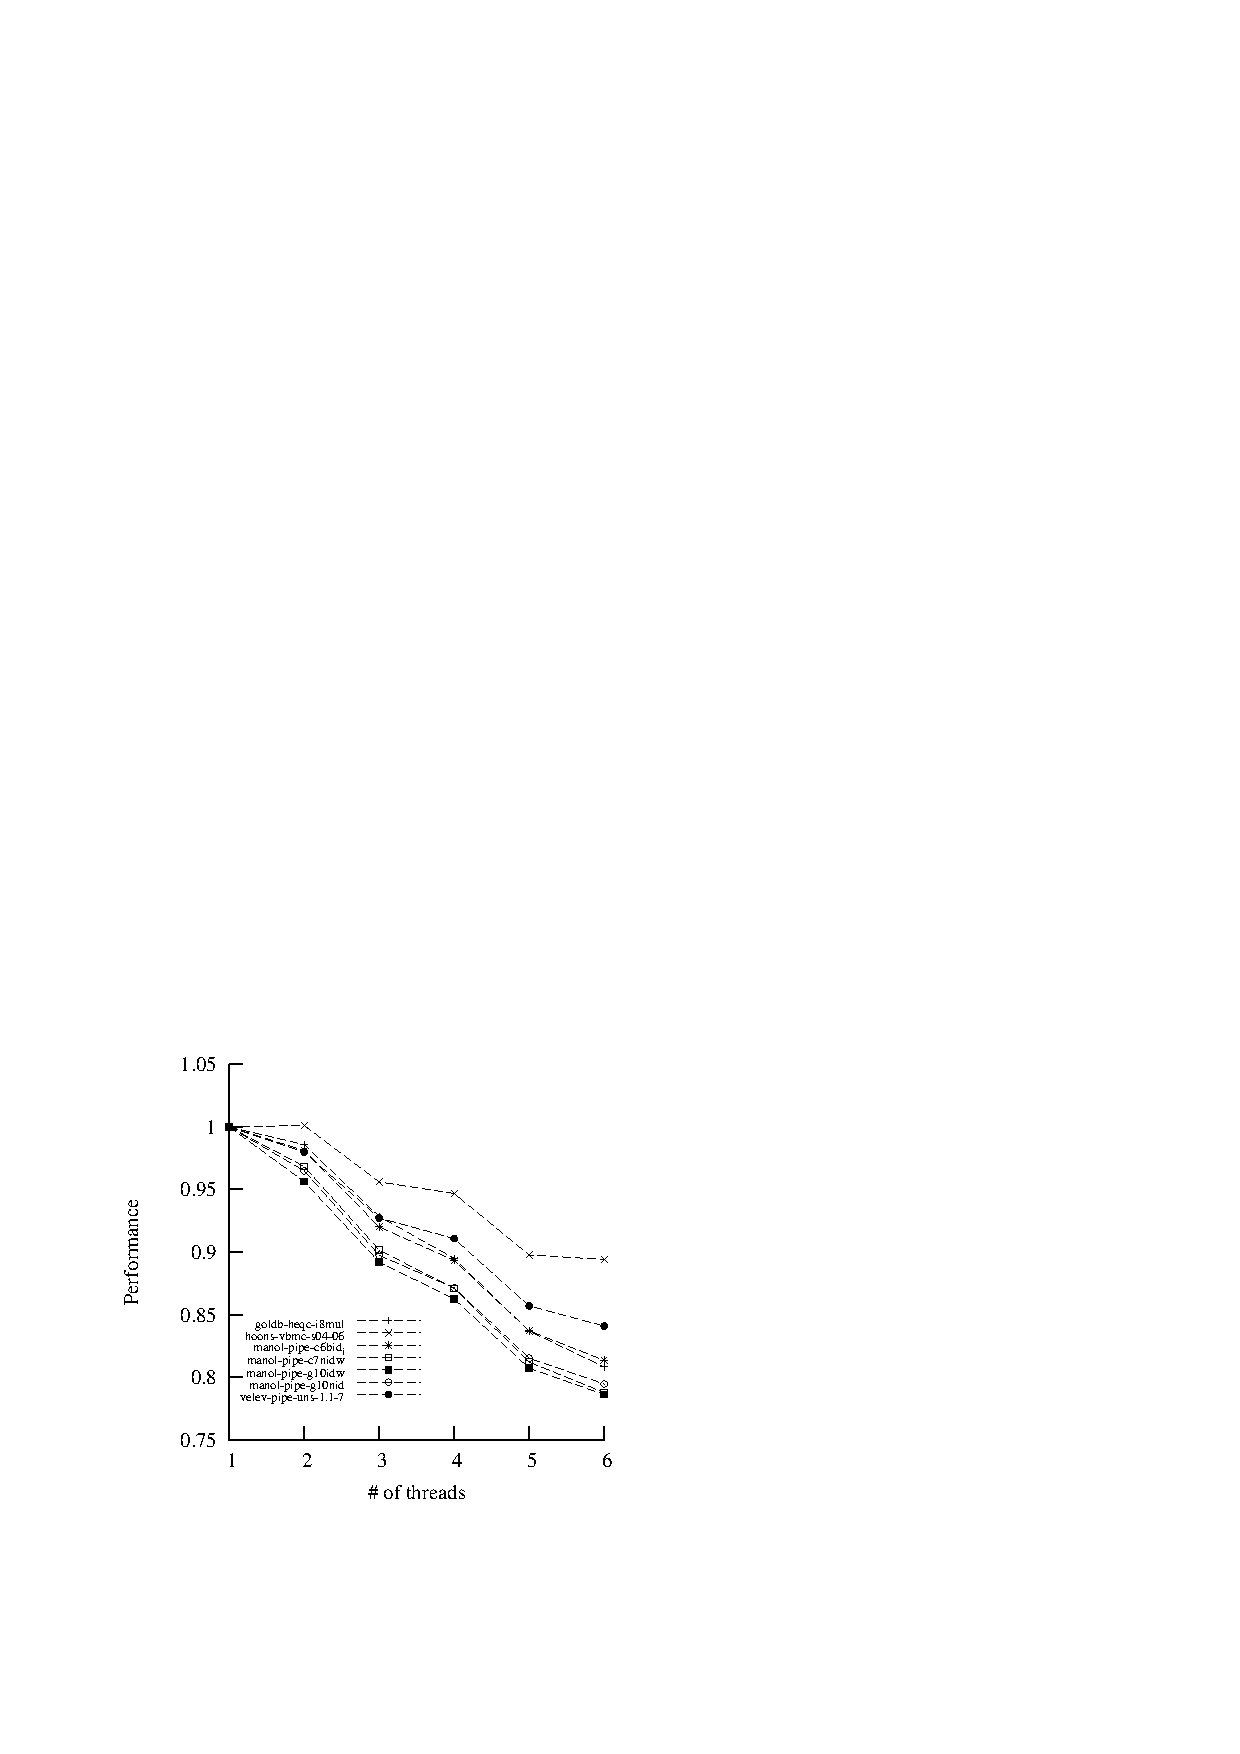
\includegraphics[scale=1]{plingeling_6cores_speedup}
  \caption{Performance decay of {\tt plingeling} when run over many cores}
  \label{fig:decay}
\end{figure}

In order to find the reason of the performance decay, we have
developed a simple portfolio-approach-based SAT solver (which we have
called AzuDICI) that allows us to both replicate the behavior of
\pling, and then also experiment with alternative scenarios (such as
sharing information among threads) in order to take measures towards
the improvement of its performance. It is important to highlight that
our SAT solver does not compare to high-performance current
state-of-the-art solvers such as \pling\ itself. AzuDICI serves as a
useful tool to test and analyze the behavior of
portfolio-approach-based SAT solvers.

%In Section \ref{} we.....

\section{Preliminaries}
\label{sec:preliminaries}
\subsection{SAT and SAT solvers}

Let $v \in V $ be a \emph{propositional variable} and $V$
 a fixed finite set of propositional symbols.  If $v \in V$,
then $v$ and $\lnot v$ are \emph{literals} of $V$.  
The \emph{negation} of a literal $l$, written $\lnot l$, denotes 
$\lnot v$ if $l$ is $v$, and $v$ if $l$ is $\lnot v$.
A \emph{clause} is a disjunction of literals $l_1 \lor\ldots\lor l_n$.
A (CNF) \emph{formula} is a conjunction of one or
more clauses $C_1 \land\ldots\land C_n$. 
 A (partial truth) \emph{assignment} $M$ is a
set of literals such that $\{ v, \lnot v \} \subseteq M$ for no $v$. A
literal $l$ is \emph{true} in $M$ if $l \in M$, is \emph{false} in $M$
if $\lnot l \in M$, and is \emph{undefined} in $M$ otherwise.  In this
paper $M$ will be written as a sequence 
 of literals with $M l$ meaning the concatenation of $M$
with $l$.   A clause $C$ is true in $M$ if at least one of its
literals is true in $M$.  It is false in $M$ if all its literals are
false in $M$, and it is undefined in $M$ otherwise. 
If $C$ is a clause $l_1
\lor\ldots\lor l_n$, we write $\lnot C$ to denote the formula $\lnot
l_1 \land\ldots\land \lnot l_n$.
A formula $F$ is true in $M$, or
\emph{satisfied} by $M$, denoted $M\models F$, if all its clauses are
true in $M$.  In that case, $M$ is a \emph{model} of $F$.  If $F$ has
no models then it is \emph{unsatisfiable}.  

The problem we are interested in is the \emph{SAT problem}: given a
formula $F$, decide whether there exists a model that satisfies $F$.
Since there exists a polynomial transformation
(see~\cite{Tseitin1968}) for any arbitrary formula to an
equisatisfiable CNF one, we will assume w.l.o.g. that $F$ is in CNF.

A software program that solves this problem is called a \emph{SAT solver}
The Conflict-Driven-Clause-Learning (CDCL) algorithm, is nowadays at the 
basis of most state-of-ther-art SAT-solvers\cite{gluclose,plingeling,cryptominisat}. 
This algorithm has, at its roots, the very 
simple DPLL algorithm~\cite{Davisetal1962CACM}. Thanks to the work done, mainly,
 in \cite{relsat,Chaff2001, GRASP1999IEEE, ZhangStickel1996IMATH, EenSorensson2003SAT,
picosat2008,} it has evolved
 to an algorithm that incorpores several conceptual and implementation 
improvements, making modern SAT-solvers able to handle formulas of millons 
of variables and clauses. In \ref{} we sketch the CDCL algorithm.

%\IncMargin{1em}
\begin{algorithm}
\SetKwData{Conflict}{conflict}
\SetKwData{Dl}{dl}
\SetKwData{Lemma}{lemma}
\SetKwData{Dec}{dec}
\SetKwData{Result}{res}\SetKwData{BV}{BV}
\SetKwInOut{Input}{Input}\SetKwInOut{Output}{Output}
\Input{formula $F=\{C_1,\ldots,C_m\}$}
\Output{SAT OR UNSAT}
 \BlankLine
  $F_w$ \assign $F$\;
  \While{true}{
    \While{\Conflict \assign PROPAGATE()}{
      \lIf{DECISION\_LEVEL == 0}{\Return UNSAT\;}
      \Lemma \assign CONFLICT\_ANALYSIS(\Conflict)\;
      \Lemma \assign LEMMA\_SHORTENING(\Lemma)\;
      LEMMA\_LEARNING(\Lemma)\;
      \Dl \assign LARGEST\_DL(\Lemma)\;
      BACKJUMP(\Dl)\;
    }
  \Dec \assign DECIDE()\;
    \lIf{ \Dec = 0 }\Return SAT\;
    DECIDE( \Dec )\;
  }
\caption{CDCL algorithm}
\label{alg:CDCL}
\end{algorithm}
%\DecMargin{1em}

As can be seen ..... explain and link concepts of the algorithm.

For a complete review of this algorithm as well as proofs over its
termination and soundness we refer to \cite{Nieuwenhuisetal2006JACM}


\subsection{Parallel SAT solvers}
Parallel SAT solvers are not as mature 
as sequential ones and it is still not clear which path to follow
when designing and implementing such new solvers.  
We mainly classify parallel SAT solvers into two categories: 
Portfolio approach solvers and divide-and-conquer ones.

The main idea behind portfolio approach solvers is the fact that different 
strategies/parameters of CDCL sequential solvers will perform better 
for different families of SAT problems. 
In sequential CDCL SAT-solving, there exist several parameters/strategies 
related with the algorithm's heuristics in, for example, restarting, deciding 
or cleaning the clause database. Taking this into 
consideration, the portfolio approach is very straightforward: 
Run a group of sequential solvers in different threads, 
each with different parameters
 and/or different strategies. The time the portfolio-approach based 
solver will take to solve the problem will be the time of the fastest 
thread in the group of solvers running in parallel. 
Differences between this kind of solvers lie in whether the clause
database should be shared~\cite{Sartagnan}, or otherwise if each thread should 
have its own database. If so, it is possible to implement the threads in order to
interchange lemmas both: aggressively~\cite{ManySAT} or selectively~\cite{plingeling} or 
not have communications between threads at all~\cite{ppfolio}.

Divide-and-conquer solvers do not try to run different solvers in parallel, 
they run one solving instance, but try to parallelize the search and divide it 
between the different threads. A common strategy to divide the search space is 
to use guiding paths~\cite{psato}. A guiding path is a partial assignment $M$ in $F$, 
which restricts the search space of the SAT problem. A solver that divides 
its search space with guiding paths will assign threads to solve $F$ with the 
given $M$ from the guiding path the thread was assigned to. Once a thread 
finishes searching a guiding path with no success, it can request another to 
keep searching (we refer to \cite{paMiraXT} for further explanations). 
Both parallelization strategies (portfolio approach and divide-and-conquer approach) 
were and are currently being applied 
to shared memory parallel computers (plingeling) as well as distributed 
memory ones~\cite{paMiraXT}. 

%As mentioned before, some parallel SAT solvers have performed at the top of the last SAT competitions, but even though they all fall into the parallel solvers category, their parallel strategies and implementations vastly differ from each other. We mainly classify parallel SAT solvers into two categories: Portfolio approach solvers and divide-and-conquer solvers.

%The main idea behind portfolio approach solvers is the fact that different kinds of sequential solvers will perform differently for different kinds of SAT problems. The most successful sequential solvers [?] all have random factors coming into play when solving SAT problems. They need random numbers for their search heuristics [?] and thus the same solver might perform very differently in two different instances of the exact same SAT problem. Taking this into consideration, the portfolio approach is a very straight forward strategy: They run a group of sequential solvers in parallel, each with different random values and/or different search strategies. The time they take to solve the problem will be the time of the fastest solver in the group of solvers running in parallel. Although all portfolio approach solvers share this same principle, they also have quite different kinds of implementations. We identify in this group the solvers that are pure portfolio approach, the ones that share clauses only logically, and the ones that share clauses physically and logically.

%Solvers which are pure portfolio approach have the most simple design. They run completely independent solvers in parallel and wait for one of them to give an answer. Despite their simplicity, the solver ppfolio [?], a pure portfolio approach solver, was the winner of the crafted and random categories, and second place in the application category of the 2011 SAT competition of parallel solvers. 

%On the other hand, we have more elaborated portfolio approach solvers, which can also share clauses logically between their different solvers [?]. One of the advantages of CDCL solvers is the fact that they can learn new lemmas as they solve a SAT problem [?]. These new lemmas will provide additional information during the solution search, so that the solver doesn't fall into previous fruitless search paths (there are also some drawbacks to adding new lemmas, which are addresses by clause database cleanups [?]). The idea is that different solvers running in parallel can share their learned lemmas so that they all benefit from what other solvers have learned and improve their own search. An example of these kind of solvers is ManySAT [?], which won the 2009 SAT competition in the parallel solver application category. ManySAT has its own sequential state-of-the-art SAT solver and runs different instances of it in parallel, using different VSIDS heuristics [?] and restart policies [?] for each of it, both of which account for random factors in the solver. The difference with pure portfolio approach solvers, is that ManySAT also shares learned lemmas between solving threads. It is called logical sharing of clauses, because the lemmas are passed as messages between threads and they never share the same physical information in memory. The advantage of logical sharing is that it is easier to implement message passing between threads, than having threads reading and modifying the same memory locations, which often requires locks that could end hindering the overall solver performance. [TALK ABOUT PLINGELING].

%Portfolio approach solvers that share clauses physically have the same strategy as mentioned before, but they share clauses by allowing threads to access the same memory locations, instead of message passing. One solver in this category is SarTagnan [?], which shares clauses logically and physically. [EXPLAIN MORE ABOUT SARTAGNAN]. 

%Divide-and-conquer solvers do not try to run different solvers in parallel, they run one solving instance, but try to parallelize the search and divide it between the different threads. A common strategy to divide the search space is to use guiding paths [?]. A guiding path is a partial assignment $M$ in $F$, which restricts the search space of the SAT problem. A solver that divides its search space with guiding paths will assign threads to solve $F$ with the given $M$ from the guiding path the thread was assigned with. Once a thread finishes searching a guiding path with no success, it can request another to keep searching. MiraXT [?] is a divide-and-conquer SAT solver which uses guiding paths. Moreover, different threads solving different guiding paths also share a common clause database, in which they store their learned lemmas. This is another example of physical clause sharing. [TALK MORE ABOUT MIRAXT]

\section{Cache performance in Plingeling}
\subsection{Memory hierarchy}
\label{sec:memhier}

For replication purposes, it is important to thoroughly characterize
the machine we are using to run the tests. All experiments were
carried out on a dual-processor 6-core Intel Xeon CPU (E5645) running
at 2.40GHz, for a total of 12 physical cores at
28.8GHz. Hyperthreading was disabled. Figure \ref{fig:topology} shows
the memory hierarchy of the testing computer. To save space, we only
show one of the chips (Socket P\#0), the other is identical.

% \begin{figure}[htp]
%   \centering
%   \includegraphics[scale=.5]{topology.pdf}
%   \caption{The memory hierarchy of the testing computer}
%   \label{fig:topology}
% \end{figure}

Each core has one processor unit (PU), with separate L1d (32KB) and L2
(256KB) caches. (The strange numbers of Cores and PUs have to do with
how the Linux Kernel sees them logically.) They share a 12MB L3
cache. Main memory is 6GB. The computer runs Linux 3.0.0-15-server, in
64-bit mode. The details of the caches are as follows:

\small
\begin{verbatim}
  L1 Data:        32K 8-way with 64 byte lines
  L2 Unified:     256K 8-way with 64 byte lines
  L3 Unified:     12288K 16-way with 64 byte lines
\end{verbatim}
\normalsize

\subsection{Experimental results}

One of the advantages we assume of parallel computing is that the more
cores we add, the better performance we will obtain. This should be
also true for plingeling, since the only difference of adding more
threads (assuming we have one thread per core) is that we will have a
greater variety of solver strategies trying to solve the problem, and
also some logical clause sharing among threads. These are all valid
assumptions in theory, but empirical results on multicore shared
memory computers also show us that increasing the number of threads
also carries a considerable decrease in performance for portfolio
solvers like plingeling.

Multicore shared memory systems have their cores sharing the same last
level cache (LLC) memory. The last level cache size in modern machines
has a few megabytes and is usually not enough to hold all the data
required by a SAT instance. Therefore, there will inevitably be some
communication between the LLC and the main memory. The time cost of
communications between the CPU and the LLC cache are much faster than
having to get the data from main memory, so we would like to keep data
transfers from main memory to a minimum.

Portfolio SAT solvers which only share clauses logically have to keep
a complete database of clauses for each thread's use. So as we add
more threads, the solver has greater needs of memory, but because all
cores share the same LLC, all threads will have a lower chance of
finding their data in the LLC as we add more threads. In this
scenario, what we would expect is to observe, as we have in our
experiments, a considerable decrease in performance when adding
threads, simply because we will incur in more LLC cache misses when
the amount of data to be manipulated by different threads
increases. We don't usually appreciate this negative performance
impact in these type of solvers, because different threads implement
different SAT solving strategies, so the solving time will mostly
depend on the fastest solving thread, shadowing the negative
performance impact of copying the clause database in each thread.

% \begin{figure}[tp]
%   \centering
%   \includegraphics[scale=1]{experiment1}
%   \caption{Performance decay of {\tt plingeling} when run over many cores}
%   \label{fig:decay}
% \end{figure}

In our experiments, we modified plingeling to replicate the exact same
search in each of its threads. What we would expect, theoretically, is
that adding more threads would have no impact in the solving time,
because all cores would be making the exact same search with their own
data. However, in practice, we found the performance decrease of
having six threads in six cores to be of around 15-40\% of the total
time one thread would take. As the LLC-load-misses (number of times
main memory data had to be retrieved) graph strongly suggests, this
performance decrease is due to the six thread solver wasting much more
time retrieving data from main memory than its single threaded version
did. As we would also expect, our results show that the L1 cache
behaves equally for each core, because L1 caches are not shared as
opposed to the LLC cache.

Another experiment that further proves our assumptions, is running
plingeling with two threads on different cores of different
CPUs. Because each CPU has its own LLC cache, we would expect in this
case to have equal performance when running one thread compared to
running two threads, which is what was observed in our measures.

\section{AzuDICI}
\label{sec:azudici}

AzuDICI\footnote{You can find the latest implementation of AzuDICI at
  \url{https://github.com/leoferres/AzuDICI}} is a standard CDCL
solver based on \pling, {\tt barcelogic} and {\tt miraXT}, built with
the aim of finding out whether or not sharing information among
threads (particularly the clauses database) helps avoid the
performance degradation that can be seen in Figure \ref{fig:decay}.

In particular, AzuDICI implements binary implication lists for the
propagation with binary clauses, and the two-watched literals scheme
for unit propagation \cite{} with clauses of more than two
literals. AzuDICI also implements the 1-UIP algorithm for conflict
analysis \ref{}, the lemma simplification algorithm used in {\tt
  PicoSAT}, Luby restarts \cite{}, a policy for lemma cleaning that
keeps only binary and ternary lemmas, and more than four-literal
lemmas that have participated in a conflict since the last
cleanup. Finally, AzuDICI also incorporates the EVSIDS heuristic for
branching literal decisions \cite{}.


\begin{figure}[tp]
  \centering
  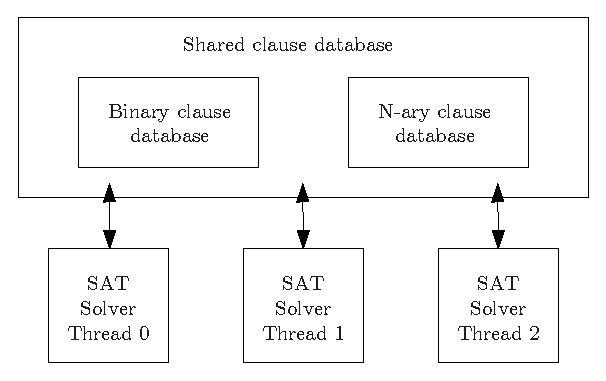
\includegraphics[scale=0.7]{AzuDICI_database}
  \caption{Shared clause database among threads.}
  \label{fig:azu database}
\end{figure}

In order to allow for comparison, we made several versions of AzuDICI.
AzuDICI-shared-all is a version which shares all clauses between
threads. It has a shared clause database which includes unitary
clauses, binary clauses and n-ary clauses (clauses with more than
two literals). Figure \ref{fig:azu database}
shows how threads share the clause database. Each thread has access
to the same physical clauses and they do not require synchronization
with each other.
Because binary implication lists are simple data structures that do
not keep track of watched literals, it is easy to share binary clauses
between threads without hindering the performance of propagation
or any other task each sequential worker thread performs. This is not
the case for the n-ary clause database. The two-watched-literal
scheme requires to make changes to the clause in order to identify
the literals being watched at one given instant (for example, place
both literals first in the clause). Since many threads will be
accessing the same clauses, these changes to the clause are not
feasible to share n-ary clauses. Instead, we have used a similar 
approach as used in
{\tt miraXT}, where each thread keeps track of the literals being
watched in each clause. Figure \ref{fig:azu design} is a
schematization of how each thread worker relates with the n-ary
clause database. Each SAT solver thread has a vector of pointers
to thread clauses called \textit{watches}, and each literal present
in the SAT problem has a position associated in this watches vector.
A thread clause has two watched literals (WL0 and WL1), two
pointers to another thread clause (NW0 and NW1) and a pointer to
an actual n-ary clause in the n-ary clause database. W0 and W1 keep
track of the literals being watched by the thread for a given n-ary
clause. NW0 and NW1 point to the next thread clauses that are also 
watching WL0 and WL1 respectively.

\begin{figure}[tp]
  \centering
  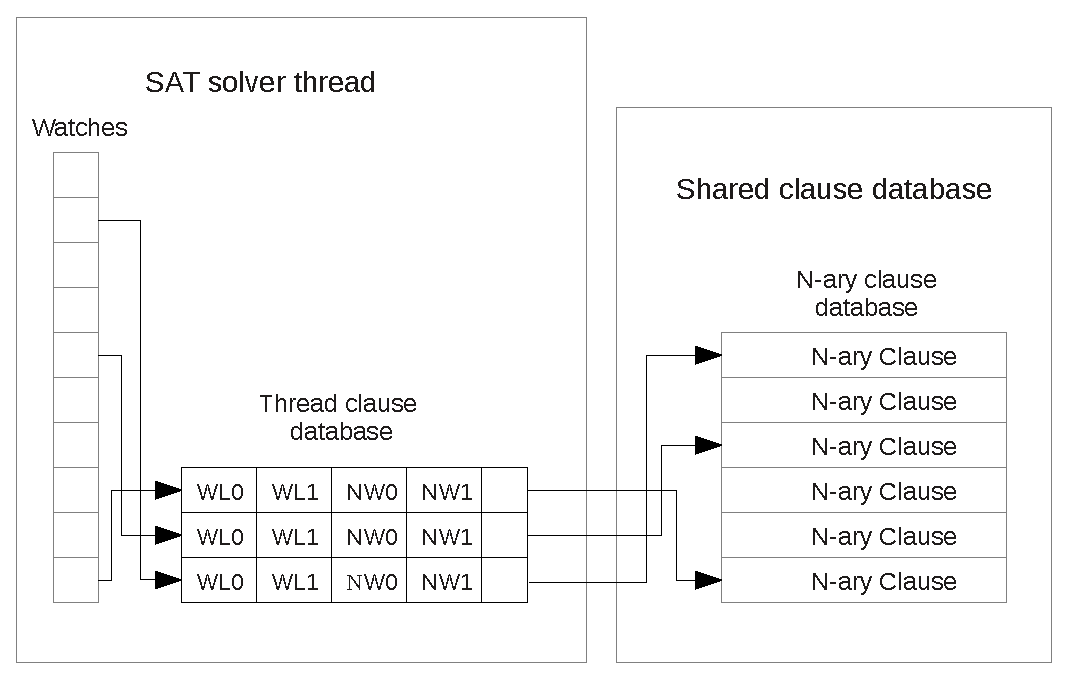
\includegraphics[scale=0.6]{AzuDICI_design}
  \caption{The thread clause database and n-ary clause database}
  \label{fig:azu design}
\end{figure}

As sharing n-ary clauses requires to make some changes to the
implementation of the propagation scheme of the two-watched-literals,
we also made the AzuDICI-shared-binaries version, which only shares
the binary clause database. With this version we aim to find out
if the drawbacks of sharing n-ary clauses, because we have to keep
track of each watched literal in each thread, surpass the benefits.
The AzuDICI-shared-none version doesn't share any clause and it's
just a group of independent solvers running in parallel, each with
its own clause database.

It is important to note that in order to make this comparison of
different solver versions objective, we have forced them all to make
the exact same search, so that the differences in performance we
observe will not be due to the search path each version takes.
For the same reason, all threads in each version of the solver will
also make the same search. We would not want an instance of a
solver performing better just because an additional thread found
a better search path.

Regarding thread safety of the solver versions which share clauses,
we added some locks to ensure the correctness of the information
being shared. The locks are only used to avoid two different threads
inserting clauses to a same clause database at the same time,
because the chance that this event occurs is so low, in practice
there is no significant contention between threads.


\section{Cache Performance in Azudici}

Experiments with AZUDICI

\section{Related Work}

Talk about miraXT and the other paper found by Leo.

\section{Conclusions and Future Work}

Let's hope to say that implementation efforts for programming a
portfolio approach-based sat-solver with shared clauseDB between
thread pays off when leading with cache problems.

Future work is to continue with the development of  azudici,
incorporating in it further enhancements like formula preprocessing,
variable elimination, etc, etc, etc.

\section*{Acknowledgments}

Acknowledgements to Barcelogic group for sharing the code of a past
Barcelogic SAT-solver and their support.

% We recommend abbrvnat bibliography style.
\bibliographystyle{splncs}

% The bibliography should be embedded for final submission.
\bibliography{bibfile}

\end{document}
